Para la problemática presentada anteriormente presentamos en esta sección: el objetivo, objetivos específicos, la justificación, el alcance y la descripción de la propuesta de solución.\\

%Definir correspondencia

\section{Objetivo}

Para mitigar las causas y reducir el impacto de los problemas que se tienen nos basamos en el siguiente objetivo: \\

Desarrollar e implementar una aplicación web para el apoyo en el control de la correspondencia del CMPL. \\

\subsection{Objetivos Específicos}

\begin{itemize}
	\item Cubrir los lineamientos establecidos para el control de correspondencia en el Manual de Procedimientos del CMPL.
	\item Tener un respaldo electrónico de los oficios y memorándums para posterior consulta.
	\item Llevar un registro de los oficios entrantes y salientes.
	\item Notificar al personal que tiene correspondencia por atender.
	\item Dar seguimiento a los asuntos que se deben atender.
\end{itemize}

\section{Justificación}
Con esto se cumple la normatividad 
%De acuerdo con los objetivos anteriores 
%Desarrollar e implementar una aplicación web que fortalezca los procesos de la administración del CMPL.

\section{Alcance}

Para presentar de mejor manera el alcance de la aplicación se divide de la siguiente manera: \\

\begin{itemize}
	\item Funcionalidad: muestra los módulos por los que estará formado la aplicación y los diferentes tipos de usuarios que la utilizarán.
	\item Plataforma: el hardware, el software y los servicios necesarios para la aplicación.
	\item Procedimiento: descripción y mejoras al procedimiento anterior.
	\item Información: la información que se va a manejar dentro de la aplicación.
	\item Propiedades de software: son los atributos con los que contará la aplicación.
	\item Interacción con el usuario: la forma en que el usuario podrá hacer el intercambio de información con la aplicación.
\end{itemize}

%%%%%%%%%% FUNCIONALIDAD %%%%%%%%%%%%
%%%%%%%%%%%%%%%%%%%%%%%%%%%%%%%%%%%%%

\subsection{Funcionalidad}

La funcionalidad la aplicación se organizará de la siguiente manera: un módulo para la gestión de usuarios, un modulo para la correspondencia interna, un módulo para la correspondencia externa. En la figura \ref{diagrama a bloques} se puede ver de manera más precisa como interactuan los bloques anteriores con los diferentes tipos de usuarios.\\

	\begin{figure}[htbp!]
		\centering
			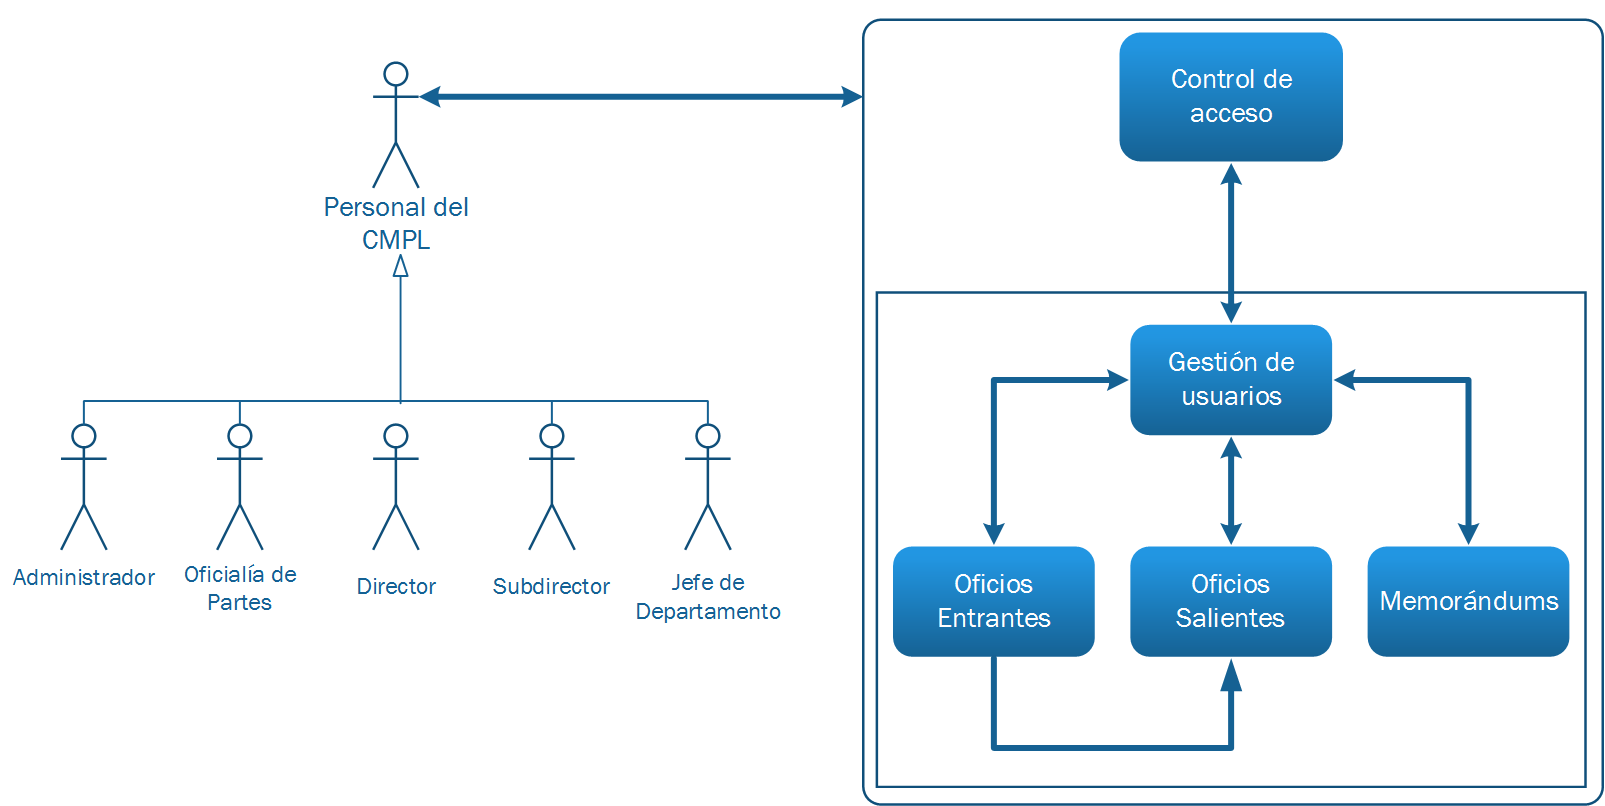
\includegraphics[width=0.8\textwidth]{images/propuesta/diagramabloques}
		\caption{Diagrama de Bloques de la Aplicación.}
		\label{diagrama a bloques}
	\end{figure}

A continuación se describe cada módulo.

\subsubsection{Módulo 1: Gestión de usuarios}
Este modulo se encargará de 
Los requerimientos considerados para este módulo son los siguientes:
\begin{itemize}
	\item Cada usuario tenga una cuenta y una contraseña de acceso.
	\item Que la aplicación controle el acceso de los usuarios restringiendo el uso de aplicación a la información y funciones que le corresponden.
	\item Cada usuario debe contar con un mecanismo para recurperar su contraseña.
	\item Cada usuario podrá editar sus datos.
\end{itemize} 

Los requerimientos funcionales que implementa este módulo son:
\begin{itemize}
	\item[RF] El usuario podrá autenticarse en la aplicación.
	\item[RF] El usuario podrá cambiar su contraseña.
	\item[RF] El usuario podrá modificar sus datos.
\end{itemize}

Con esto se resuelve la problemática de el acceso a información confidencial ya que existen documentos con información de ese tipo que era para una persona y en ocasiones era vista por personal no autorizado.

%Con lo anterior se resuelve que el usuario sólo acceda a la información que le corresponda, con las funciones que correspondan de acuerdo al tipo de usuario que sea.

%Los requerimientos considerados para este módulo son los siguientes:
\begin{itemize}
	\item Registrar nuevos usuarios.
	%\item Editar los datos de los usuarios.
	\item Dar de baja a los usuarios.
	\item Consultar los usuarios registrados.
\end{itemize}

Los requerimientos funcionales que implementa este módulo son:
\begin{itemize}
	\item[RF] Registrar nuevos usuarios.
	\item[RF] Dar de baja a usuarios.
	\item[RF] Consultar los usuarios registrados
\end{itemize}

Con esto se resuelve la problemática de ...

\subsubsection{Modulo 3: Correspondencia Externa}
Los requerimientos considerados para este módulo son los siquientes:

\begin{itemize}
	\item Consultar los oficios que se le han envíado.
	\item Consultar los oficios o memorándums que ha envíado.
	\item Consultar el estatus de cada oficio.
	\item Dar el seguimiento a cada oficio.
	\item Turnar o envíar copia a otro usuario.
	\item Registrar cuando llega un nuevo oficio.
	\item Tener un respaldo del oficio.
	\item Saber el momento de que se envíe un oficio o memorándum.
\end{itemize}

\subsection{Modulo 4: Correspondencia Interna}

Los requerimientos funcionales que implementa este módulo son:
\begin{itemize}
	\item[RF] El usuario podrá registrar oficios entrantes.
	\item[RF] El usuario podrá guardar el documento escaneado.
	\item[RF] El usuario podrá enviar una copia.
	\item[RF] El usuario podrá cancelar el proceso de la correspondencia.
	\item[RF] El usuario podrá registrar anexos.
\end{itemize}

Con esto se resuelve la problemática de que para los oficios y memorándums: se lleve de manera adecuada su registro, se tenga un respaldo, se le de el seguimiento adecuado a cada uno (la notificación a cada usuario cuando reciba correspondencia, el estatus de cada uno).
%De acuerdo con los requerimientos anteriores se resuelve que: los oficios tengan un respaldo, que se sepa el estatus de un oficio, que se lleve de manera correcta el registro de los oficios y que se le notifique al usuario que ha recibido correspondencia.\\

En cuanto a los tipos de usuarios que utilizarán la aplicación, cada uno tiene responsabilidades diferentes en el CMPL por lo tanto dentro de la aplicación sus funciones serán diferentes y se describen a continuacion: \\
%%%%%%%%%%%%%%%%%%%%%%%%%%%%%%%%%%%%%%%%%%%%%
%%%%%%%%%%%%%%%%%ROLES DE USUARIOS%%%%%%%%%%%
\subsection{Descripción de roles de usuarios}
En esta sección describimos cada uno de los posibles perfiles de usuarioslll
\subsubsection{Administrador}
Es el jefe del Departamento de Sistemas y Banco de Datos del CMPL. Tiene el control total de la administración de la información mostrada en la aplicación web.\\

\textbf{Responsabilidades:}
\begin{itemize}
	\item Dar de alta nuevos usuarios.
	\item Editar usuarios existentes.
	\item Eliminar usuarios.
	\item Registrar correspondencia saliente (oficios y memorándums).
	\item Consultar correspondencia.
	\item Dar seguimiento a su correspondencia.
\end{itemize}

\subsubsection{Oficialía de Partes}
Es la persona que lleva a cabo la recepción de correspondencia formal del CMPL. Recibe los documentos de correspondencia y los registra en una bitácora; firma y sella de recibido y turna los oficios y memos a sus respectivos destinatarios.\\

\textbf{Responsabilidades:}
\begin{itemize}
	\item Verificar que los documentos recibidos cumplan con todos los lineamientos requeridos para su recepción.
	\item Registrar la correspondencia formal interna y externa del CMPL.
	\item Turnar los oficios y memorándums a sus respectivos destinatarios.
	\item Registrar correspondencia saliente.
\end{itemize}

\subsubsection{Personal CMPL}
Es un trabajador del CMPL registrado en el directorio, que no es Jefe del Departamento de Sistemas y Banco de Datos o encargado de Oficialía de Partes.\\

\textbf{Responsabilidades:}
\begin{itemize}
	\item Checar su correspondencia entrante.
	\item Registrar correspondencia saliente.
	\item Turnar correspondencia.
	\item Recibir correspondencia.
	\item Atender observaciones a los oficios registrados.
\end{itemize}

\subsubsection{Director}
Es un trabajador del CMPL con el nombramiento de “Director”. Es la persona que representa al centro ante otras dependencias. Se encarga de administrar y gestionar las decisiones importantes del centro junto con su grupo de trabajadores.\\

\textbf{Responsabilidades:}
\begin{itemize}
	\item Turnar oficios entrantes.
	\item Turnar copia de oficios entrantes.
	\item Firmar oficios salientes.
	\item Cancelar proceso de oficios entrantes.
	\item Cancelar proceso de oficios salientes.
	\item Ver detalles de correspondencia.
	\item Responder oficios.
\end{itemize}

\subsubsection{Jefe de Departamento}
Es un trabajador del CMPL que está como encargado de alguna de las diferentes jefaturas que existen en el centro. Se encarga de apoyar a la dirección con las decisiones importantes para el CMPL y de atender los asuntos que conciernen con el departamento del cual está encargado.\\

\textbf{Responsabilidades:}
\begin{itemize}
	\item Atender correspondencia a nombre del director.
	\item Manejar los indicadores mensuales.
	\item Cancelar proceso de correspondencia saliente.
	\item Generar oficios salientes nuevos.
	\item Dar respuesta a oficios entrantes.
	\item Atender observaciones a los oficios registrados.
\end{itemize}

\subsubsection{Subdirector}
Es un trabajador del CMPL que esta como encargado en alguna de las subdirecciones existentes dentro del centro. Se encarga de las decisiones que conciernen al área y de la administración de dicho departamento. Puede que tenga a su cargo otra jefatura y debe trabajar en conjunto con esta otra área.\\ 

\textbf{Responsabilidades:}
\begin{itemize}
	\item Responder oficios entrantes.
	\item Registrar oficios salientes.
	\item Turnar correspondencia en caso de que tenga alguna jefatura a su cargo.
	\item Ver detalles de correspondencia.
	\item Atender observaciones a los oficios registrados.
\end{itemize}

%%%%%%%%%% PLATAFORMA %%%%%%%%%%%%%%%
%%%%%%%%%%%%%%%%%%%%%%%%%%%%%%%%%%%%%
\subsection{Plataforma}

Para que la aplicación funcione se necesita de los componentes de hardware, software y los servicios necesarios con el fin de que funcione.\\
\subsubsection{Hardware, Software y Servicios}

Dentro del hardware se requiere que el CMPL cuente con un servidor para que de el servicio a otras máquinas y que el personal cuente con una computadora (de escritorio o laptop) con conexión a internet. A su vez cada usuario con su respectiva computadora requiere de un explorador de internet ya sea Chrome, Mozilla, Safari, entre otros.\\

Por último se requiere de los siquientes servicios: 
\begin{itemize}
	\item Energía eléctrica o una planta de luz para que cuando se vaya la luz el servidor siga operando.
	\item Aire acondicionado: para que no se caliente el servidor.
	\item Site: para colocar el servidor.
	\item Seguridad física: para que ninguna persona diferente al jefe del departamento de sistemas y banco de datos modifique la configuración del servidor.
	\item Servicio web: para que los usuarios accedan a la aplicación. 
\end{itemize} 

En la figura \ref{arquitectura} se puede ver de manera más precisa como interactuan los servicios anteriores con los usuarios.\\

	\begin{figure}[htbp!]
		\centering
			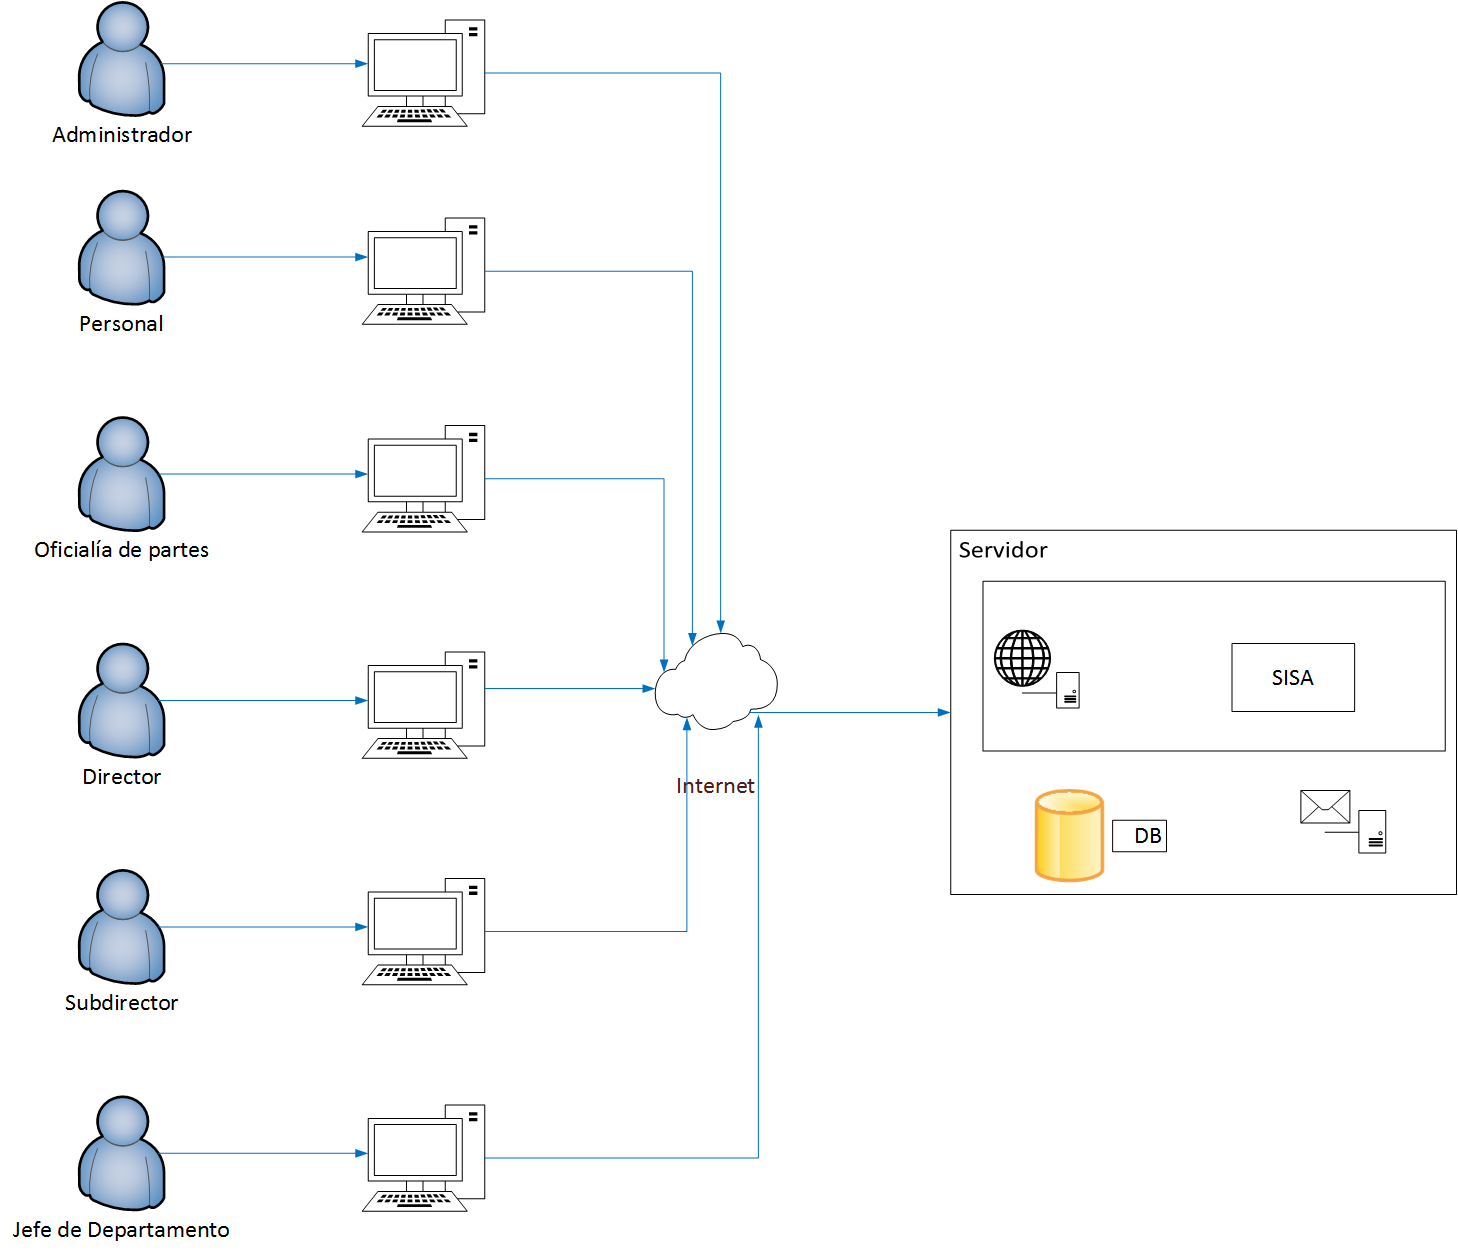
\includegraphics[width=0.8\textwidth]{images/propuesta/arquitectura}
		\caption{Arquitectura de la Aplicación.}
		\label{arquitectura}
	\end{figure}
	
%%%%%%%%%% PROCEDIMIENTO %%%%%%%%%%%%
%%%%%%%%%%%%%%%%%%%%%%%%%%%%%%%%%%%%%
\subsection{Procedimiento}
Con esta propuesta se mejora el procedimiento presentado en el capitulo 1, las principales mejoras son:
\begin{itemize}
	\item Alertas al usuario: cuando el usuario este utilizando la aplicación está mostrará los asuntos que no ha atendido. 
	\item Notificaciones al correo: una vez que se turne un oficio, se enviará un correo electrónico al usuario diciendo que tiene un nuevo asunto por atender. 
	\item Respaldos: 
	\item Seguimiento: 
\end{itemize}


%%%%%%%%%% INFORMACION %%%%%%%%%%%%%%
%%%%%%%%%%%%%%%%%%%%%%%%%%%%%%%%%%%%%
\subsection{Información}

Para la información a manejar dentro de la aplicación de manera general se comtempla manejar la información de:
\begin{itemize}
	\item Usuarios: Nombre completo, departamento al que pertenece y rol que desempeña dentro de la aplicación.
	\item Documentos: número de oficio, fecha de redacción, área que emite, emisor, cargo del emisor, destinatario, cargo del destinatario, dependencia, asunto, fecha de acuse, nombre de quien entrega y si requiere o no respuesta. Además contará con un selector de archivos que permite la carga del documento escaneado en formato PDF y adjuntarlo al registro.
\end{itemize}

%%%%%%%%%% PROPIEDADES DE SW %%%%%%%%
%%%%%%%%%%%%%%%%%%%%%%%%%%%%%%%%%%%%%
\subsection{Propiedades de software}

\textbf{Confiabilidad\\}
La confiabilidad de un sistema es la probabilidad de que el sistema realizará su funcionalidad bajo los limites de diseño especificados, sin fallo, durante un periodo de tiempo determinado. \\

\textbf{Disponibilidad\\}
La disponibilidad es la probabilidad de que el sistema esta operando en un tiempo particular.\\ 

\textbf{Robustes\\}
Un sistema de software es robusto si es capaz de responder adecuadamente a las condiciones de tiempo de ejecución no anticipados.\\


%%%% INTERACCION CON EL USUARIO %%%%%
%%%%%%%%%%%%%%%%%%%%%%%%%%%%%%%%%%%%%
\subsection{Interacción con el usuario}

Cuenta con una pantalla que tiene un formulario de autenticación donde se le solicita al usuario su correo institucional y su contraseña. Cuando el usuario ingresa sus credenciales la aplicación verifica su correo y su contraseña; si existen entonces la aplicación muestra la pantalla principal de acuerdo al tipo de usuario que sea. En caso contrario, la aplicación regresa a la pantalla de autenticación con un mensaje de error diciendo que los datos introducidos no son válidos.

\section{Metodología}

